\begin{ZhChapter}

\chapter{實驗結果與分析}

\section{實驗環境與參數設計}

本研究實驗環境包含實體硬體測試平台與模擬環境平台兩部分,搭配修改後之 FruityMesh 協定,用以驗證所提出之拓樸生成與傳輸優化機制在不同環境下的效能表現。

\subsection{實體實驗平台}
實體網路建構基於 Nordic nRF52840 SoC 開發板,相關配置如表\ref{tab: 實體實驗平台配置}所示。

\begin{table}[H]
\centering
\caption{實體實驗平台配置}
\label{tab: 實體實驗平台配置}
\begin{tabular}{|c|c|}
    \hline
    項目 & 說明 \\ 
    \hline
    晶片型號 & Nordic Semiconductor nRF52840(支援 BLE 5.0) \\
    \hline
    節點數量 & 共 6 個節點(含 1 個 Sink 節點) \\
    \hline
    資料傳輸通道 & 使用 USB 作為 Log 回傳通道 \\
    \hline
    電力供應方式 & 透過 USB 供電進行情境部署 \\
    \hline
    節點與節點距離 & 小於1公尺 \\
    \hline
\end{tabular}
\end{table}

本研究所進行的實體實驗平台建置於 Nordic Semiconductor 所推出的 nRF52840-DK 開發板上,整體平台共由 6 個 nRF52840 節點組成,包含一個 Sink 節點與多個子節點的 BLE Mesh 結構。為驗證所提出之網路拓樸建立機制與封包調度策略在實際硬體環境中的效能與穩定性,實驗於室內空間中進行部署,如圖 \ref{fig: nRF52840開發板擺放示意圖} 所示。所有開發板節點平均間距小於 1 公尺,並皆透過 USB 介面連接至電腦,作為穩定的 5V 電源來源,同時也用於傳輸日誌資料(Log),可即時監控封包的發送、接收與轉發過程。透過此小規模實體實驗,可進一步驗證本研究所設計之機制的實用性與真實應用潛力。

%本研究所進行的實體實驗平台建置於 Nordic Semiconductor 所推出的 nRF52840-DK 開發板上,整體平台共由 6 個 nRF52840 節點組成。我們首先模擬 Sink 節點與多個子節點,再透過實際部署驗證所提出之拓樸建立機制與封包傳輸策略在真實硬體環境下的效能表現。

%為驗證所提出之網路拓樸與封包調度機制的實用性與穩定性,本研究於室內空間中建置 nRF52840-DK 開發板進行小規模實體實驗,如圖\ref{fig: nRF52840開發板擺放示意圖}所示。實驗部署共使用六片 nRF52840-DK 開發板,節點間平均距離均小於 1 公尺。每片開發板皆透過 USB 介面與電腦連接,不僅提供 5V 穩定電源供應,同時作為日誌資料 (Log) 傳輸通道,以即時監控節點間封包的發送、接收與轉發過程。

\begin{figure}[H]
  \centering
  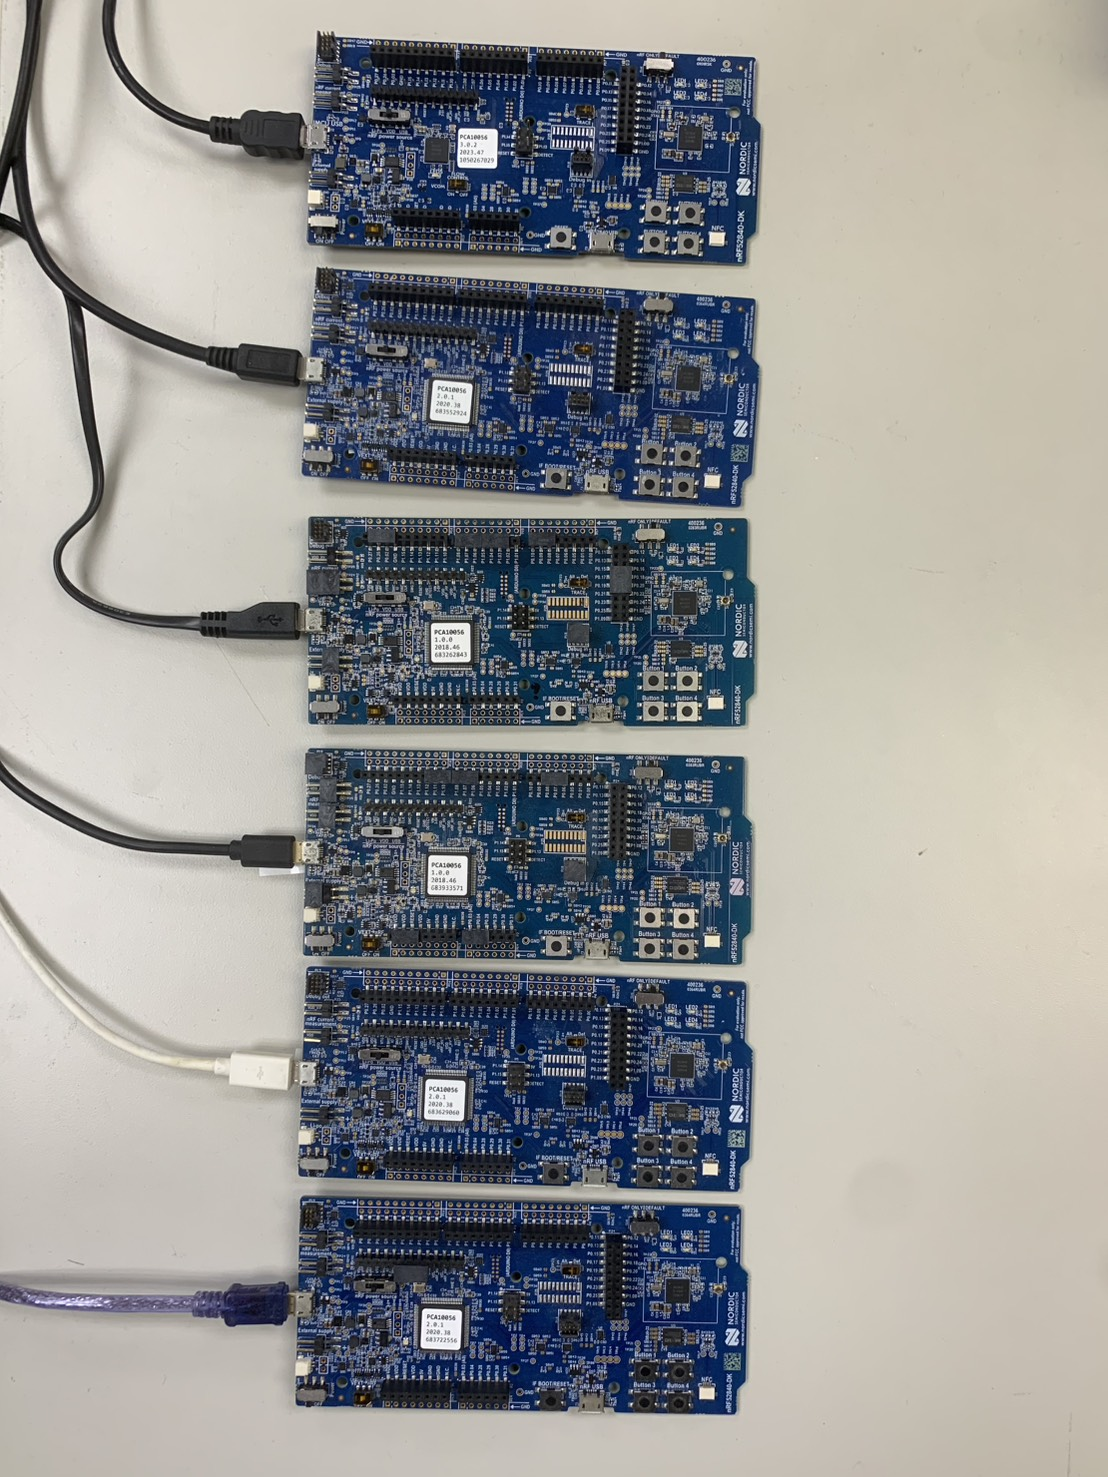
\includegraphics[width = 0.8\textwidth]{image/nRF52840開發板擺放示意圖.jpg}
  \caption{nRF52840-DK 開發板實體部署示意圖}
  \label{fig: nRF52840開發板擺放示意圖}
\end{figure}

電腦端亦搭配Putty工具,可視化封包流動與節點行為,有助於分析封包延遲、重傳次數與拓樸變化等網路效能指標。各節點皆搭載 Nordic 所提供之 SoftDevice BLE 堆疊,並以 FruityMesh 為基礎韌體框架進行修改與擴充。根據不同實驗目的,調整拓樸建立參數、連線策略與角色排程機制,並透過USB燒錄至各 nRF52840-DK 板上進行測試。透過 Putty 工具紀錄各節點狀態與封包交換資訊,如圖\ref{fig: nRF52840-DK日誌紀錄},觀察節點之間的拓樸變化與網路重建過程。

\begin{figure}[H]
    \centering
    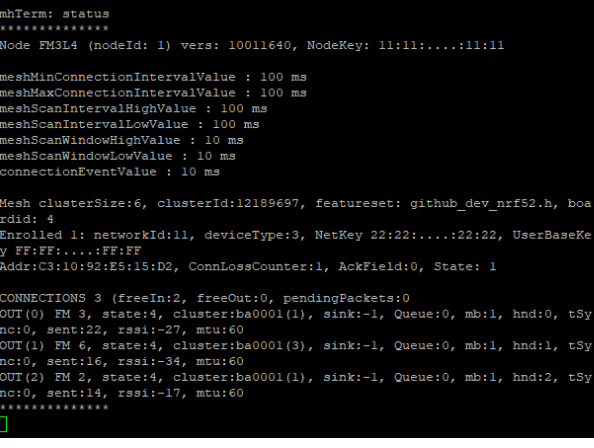
\includegraphics[width = 0.8\textwidth]{image/UART日誌紀錄.png}
    \caption{nRF52840-DK日誌紀錄}
    \label{fig: nRF52840-DK日誌紀錄}
\end{figure}

%實體節點部署於室內空間中,模擬感測器佈建情境。節點間距為 小於 1 公尺。所有實驗皆重複進行多次以確保結果穩定與具參考性,並與模擬平台結果進行對比分析,以佐證演算法之可行性與實用性。

\subsubsection{實體實驗平台的同步機制}

本研究實體實驗同步機制主要參考\cite{112TIT00392032}所提出之 BLE Mesh 網路時間同步設計,其方法透過兩階段進行節點 RTC 時間同步,包括初次同步之 TIMESYNC 封包與後續誤差校正之 CORRECTION 封包。有效提升分層資料傳輸之整體穩定性與時效性。

然而在本實驗實施過程中,觀察到一個在實體部署條件下額外產生的問題,當同步過程完成後,若使用者透過 Terminal 輸入控制指令(Command)至某一節點,該節點因進入處理指令流程而暫時中斷 RTC 計數與資料傳輸,進而導致與其他節點間再次產生時間差異,影響同步準確性與傳輸效能。

為避免此現象,本研究對時間同步流程進行優化調整。當整個BLE Mesh同步完成後,於預先設定的時間點,由 Sink 節點主動廣播啟動封包傳送的通知。各個節點接收通知後,不用再等待手動下指令,將會自動傳送封包至 Sink節點,從而避免因人工介入造成的延遲與時間偏移,有效維持整體網路節點間的同步性。

該方法不僅維持了原有 CORRECTION 封包的時間校正精度,更兼顧實體實驗中人為操作介入所帶來的同步中斷風險,使得實驗平台下的時間管理更加穩健可靠。


\subsection{模擬實驗平台(CherrySim)}
為進一步驗證系統在大規模節點下的可擴展性與穩定性,本研究亦使用 CherrySim 模擬器進行測試。 CherrySim 作為模擬 BLE 網路的主要工具。CherrySim 是由 FruityMesh 開發團隊所提供的官方模擬器,能夠在不需要實體硬體的情況下,模擬基於 Nordic nRF52 系列晶片及其 SoftDevice 堆疊的 BLE 節點行為。CherrySim 支援完整的連線協定模擬,包含封包交換、連線建立、訊號強度 (RSSI)、連線參數(如 CE/CI)等,並提供豐富的除錯與日誌紀錄功能。

此外,CherrySim 內建 網路狀態視覺化介面,可清楚顯示模擬過程中節點的地理分布與連線拓樸,並即時更新節點之間的連線變化。研究人員可透過該介面直觀掌握拓樸建立流程、連線演化過程與自我修復行為。

\subsubsection{模擬實驗流程}
本研究於 CherrySim 中設計三組模擬情境,分別模擬節點數為 11、21 及 31 的藍牙網路環境,每種情景分別使用3種不同seed進行模擬。每組模擬皆包含一個 Sink 節點,並配置節點4的位置為Sink點,模擬其拓樸自動生成與穩定過程,模擬觀察拓樸建立完成所需時間、自我修復機制及平均 HopsToSink 數值。

其中,11節點網狀節點配置示意圖,如圖\ref{fig: 模擬實驗11點網狀節點配置示意圖}所示,21節點網狀節點配置示意圖,如圖\ref{fig: 模擬實驗21點網狀節點配置示意圖}所示,31節點網狀節點配置示意圖,如圖\ref{fig: 模擬實驗31點網狀節點配置示意圖}所示。

\begin{figure}[H]
    \centering
    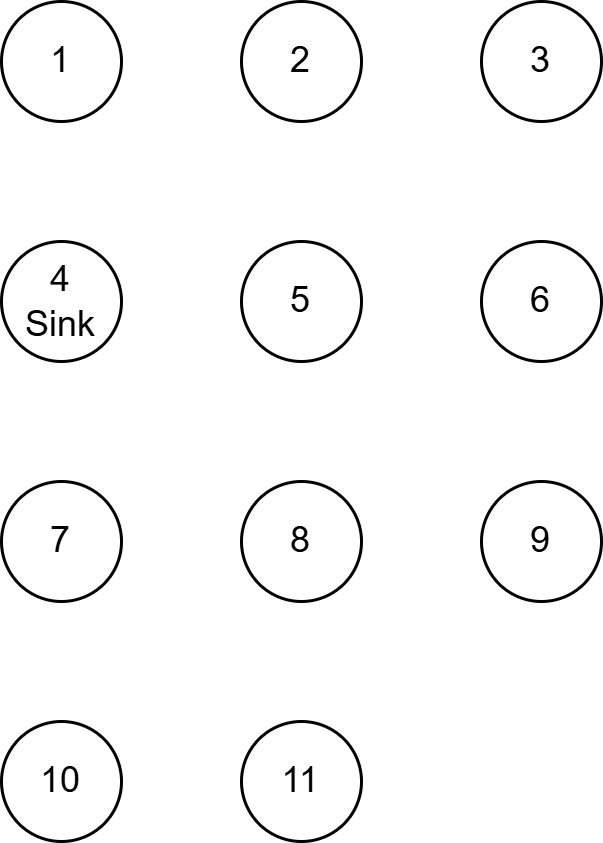
\includegraphics[width = 0.3\textwidth]{image/模擬實驗11點網狀節點配置示意圖.png}
    \caption{模擬實驗11點網狀節點配置示意圖}
    \label{fig: 模擬實驗11點網狀節點配置示意圖}
\end{figure}

\begin{figure}[H]
    \centering
    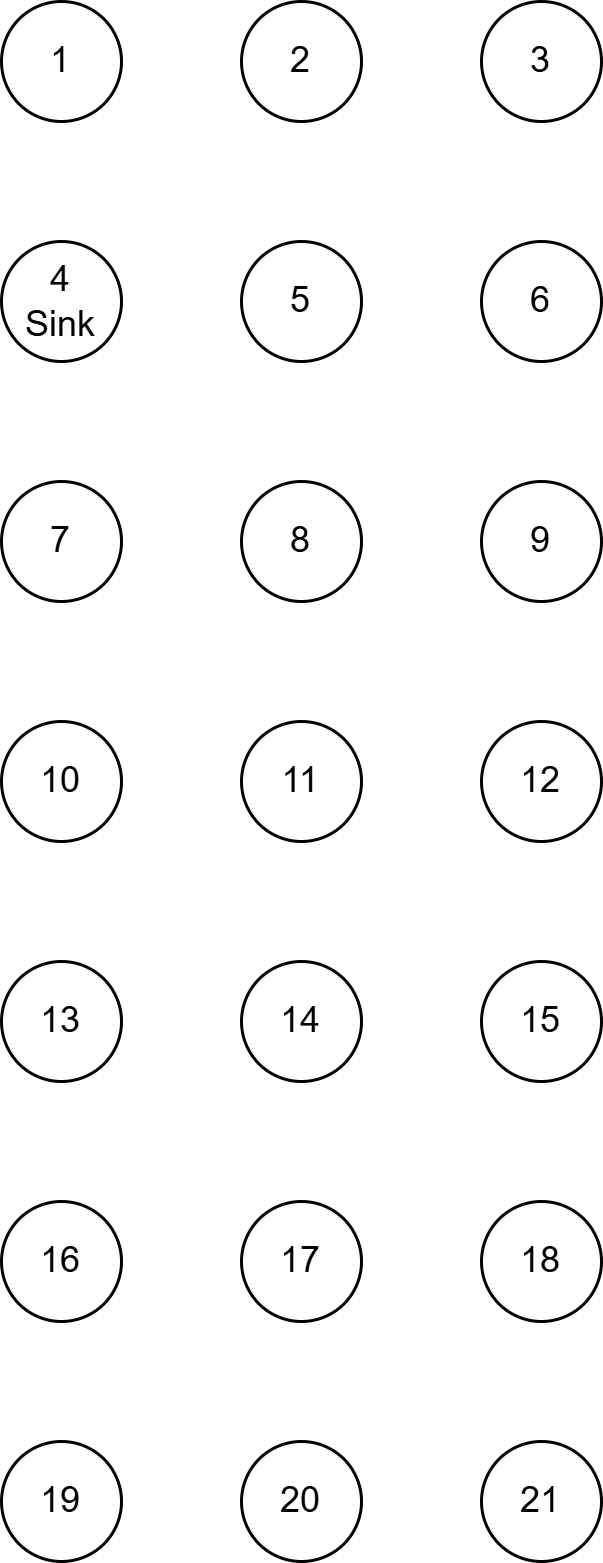
\includegraphics[width = 0.3\textwidth]{image/模擬實驗21點網狀節點配置示意圖.png}
    \caption{模擬實驗21點網狀節點配置示意圖}
    \label{fig: 模擬實驗21點網狀節點配置示意圖}
\end{figure}

\begin{figure}[H]
    \centering
    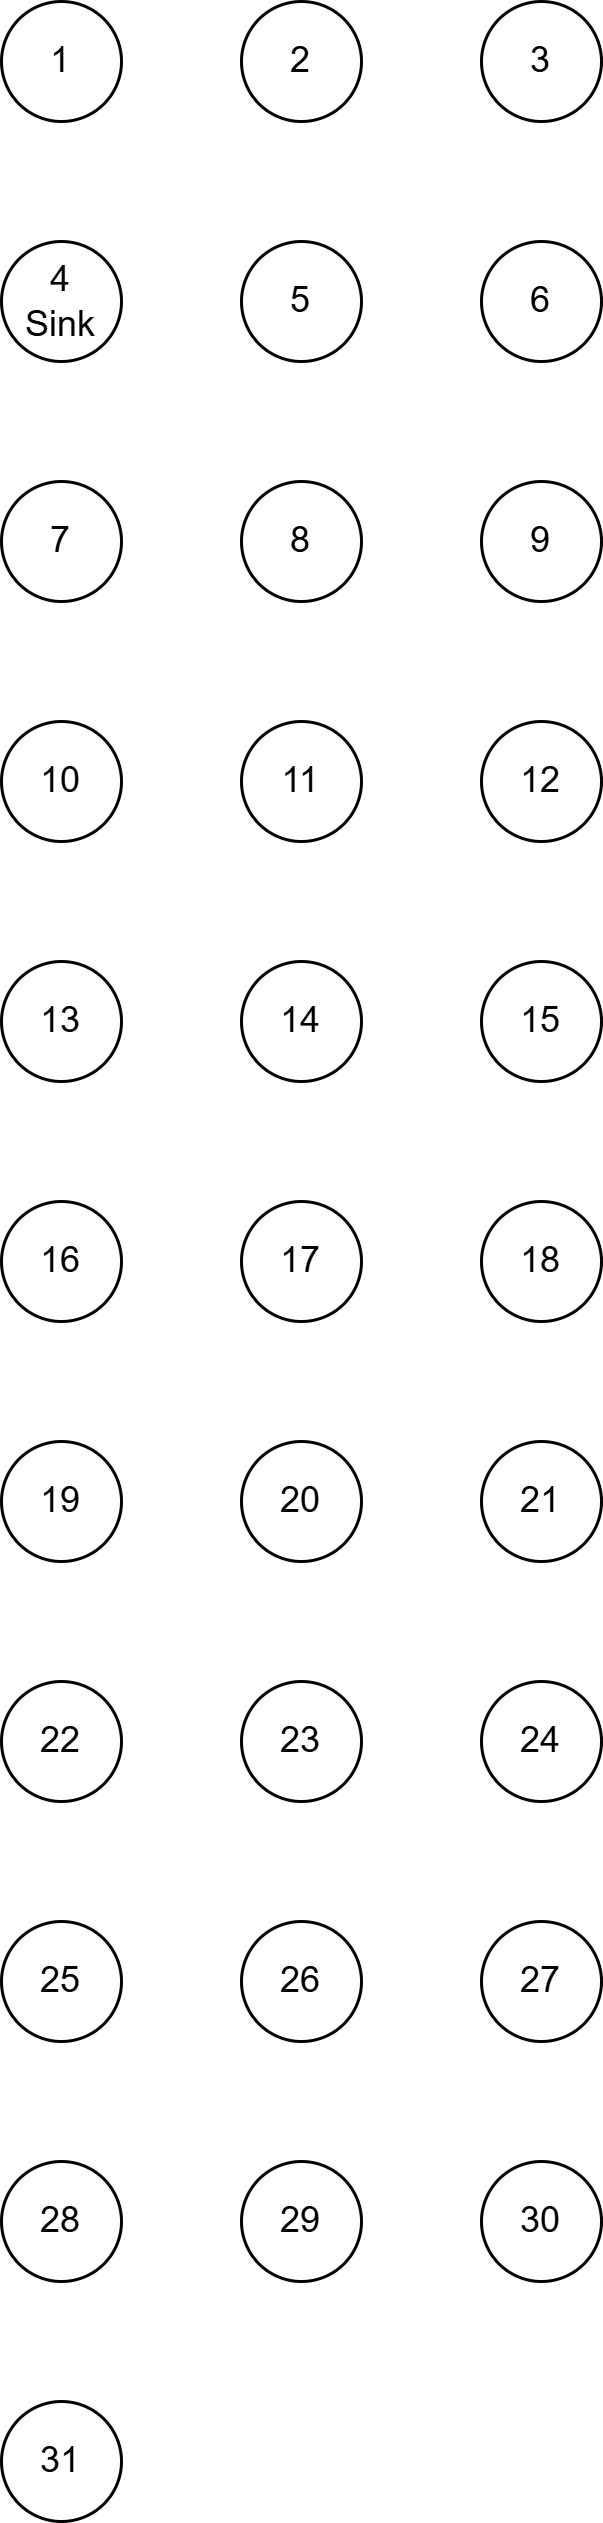
\includegraphics[width = 0.3\textwidth]{image/模擬實驗31點網狀節點配置示意圖.png}
    \caption{模擬實驗31點網狀節點配置示意圖}
    \label{fig: 模擬實驗31點網狀節點配置示意圖}
\end{figure}

\subsubsection{模擬實驗參數設定}
模擬實驗中,所有節點相關參數如表\ref{tab: 模擬實驗參數設定表}所示。表中包含Simulated Device、Node Deployment、Distance between nodes、節點數量、Sink 節點位置、Seed、Connection Interval 及 Connection Event 等參數設定。

\begin{table}[H]
    \centering
    \caption{模擬實驗參數設定表}
    \label{tab: 模擬實驗參數設定表}
    \begin{tabular}{|c|c|}
        \hline
        參數名稱 & 設定值 \\
        \hline
        Simulated Device & nRF52DK \\
        \hline
        Node Deployment & Grid \\
        \hline
        Distance between nodes & 3m \\
        \hline
        節點數量 & 11, 21, 31(including 1 sink node) \\
        \hline
        Sink 節點位置 & 節點4 \\
        \hline
        Seed & 1, 10, 100 \\
        \hline
        Connection Interval & 100 ms \\
        \hline
        Connection Event &  10 ms  \\
        \hline
    \end{tabular}
\end{table}

\section{效能評估指標}
本研究針對所提出的拓樸生成與傳輸優化機制,設計以下數項效能評估指標,以量化系統在不同模擬情境下的表現。

\subsection{拓樸建立時間}
拓樸建立時間是指系統成功建立 Mesh 拓樸所需的時間。此指標反映系統在節點加入網路時的效率,時間越短表示系統越能快速適應新節點,具備更佳的擴展性與部署靈活性,如\ref{eq: TopologyEstablishmentTime}式所示。

\begin{equation}
\label{eq: TopologyEstablishmentTime}
\text{TopologyEstablishmentTime} = Topology_{finish} - Topology_{init}
\end{equation}
其中:
\begin{itemize}
    \item $Topology_{finish}$ 為拓樸建立完成的時間點。
    \item $Topology_{init}$ 為拓樸建立開始的時間點。
\end{itemize}

\subsection{自我修復時間}
自我修復時間指的是節點在斷線後,能夠重新加入網路並恢復傳輸功能所需的時間。此指標評估網路面對節點失效或路徑中斷時的容錯能力與恢復效率,能顯示出 Mesh 結構的穩定性,如\ref{eq: SelfHealingTime}式所示。

\begin{equation}
\label{eq: SelfHealingTime}
\text{SelfHealingTime} = Topology_{finish} - Node_{disconnection}
\end{equation}

其中:
\begin{itemize}
    \item $Topology_{finish}$ 為拓樸建立完成的時間點。
    \item $Node_{disconnection}$ 為節點斷線的時間點。
\end{itemize}

\subsection{平均 HopsToSink 數值}
平均 HopsToSink 表示封包從任意節點傳送至 Sink 節點所需的平均跳數。此數值越低代表網路拓樸越扁平,資料傳輸的路徑越短,能有效降低延遲並提升整體效率,如\ref{eq: AvgHopsToSink}式所示。

\begin{equation}
\label{eq: AvgHopsToSink}
\text{AvgHopsToSink} = \frac{\sum HopsToSink}{N_{nodes}}
\end{equation}

其中:
\begin{itemize}
    \item $\sum HopsToSink$ 為所有節點到 Sink 節點的跳數總和。
    \item $N_{nodes}$ 為網路中節點的總數,不包含Sink節點。
\end{itemize}

\subsection{平均封包傳輸延遲}
此指標衡量封包從來源節點產生到 Sink 節點成功接收所經歷的時間總和,反映網路整體的即時性與處理能力,此值越低,代表網路回應時間越短、傳輸效率越高。如\ref{eq: AvgPacketDelay}式所示。
\begin{equation}
\label{eq: AvgPacketDelay}
\text{AvgPacketDelay} = \frac{\sum Delay_{end-to-end}}{\sum N_{sink\_received\_packet}}
\end{equation}

其中:
\begin{itemize}
    \item $\sum Delay_{end-to-end}$ 為所有成功接收封包從來源節點產生至 Sink 節點接收之總延遲時間。
    \item $\sum N_{sink\_received\_packet}$ 為所有成功接收封包的總數。
\end{itemize}

\subsection{平均封包抵達率}

平均抵達率(Average Packet Delivery Ratio, PDR)表示成功接收封包的總數,佔來源節點原本應發送封包總數的比例,當網路品質下降或傳輸負載過高時,PDR 會明顯降低,如\ref{eq: AvgPDR}式所示。

\begin{equation}
\label{eq: AvgPDR}
\text{AveragePDR} = \frac{\sum N_{sink\_received\_packet}}{\sum N_{source\_send\_packet}} \times 100\%
\end{equation}

其中:
\begin{itemize}
    \item $\sum N_{sink\_received\_packet}$ 為所有成功接收的封包數量。
    \item $\sum N_{source\_send\_packet}$ 為所有來源節點發送的封包數量。
\end{itemize}

\subsection{平均封包重傳率(Average Retransmission Rate)}

平均重傳率衡量封包在網路中被重複傳送的比例,反映網路壅塞或角色衝突導致的傳輸效率問題,重傳率越低,代表網路越穩定、資源使用效率越高,如\ref{eq: AvgRetransmissionRate1}式及\ref{eq: AvgRetransmissionRate2}式所示。

\begin{equation}
\label{eq: AvgRetransmissionRate1}
\text{AvgRetransmissionRate} = \frac{\sum RetransmissionPacket}{\sum Conn_{expect\_send\_packet}} \times 100\%
\end{equation}

\begin{equation}
\label{eq: AvgRetransmissionRate2}
\sum RetransmissionPacket = \sum Conn_{actual\_send\_packet} - \sum Conn_{expect\_send\_packet}
\end{equation}

其中:
\begin{itemize}
    \item $\sum Conn_{expect\_send\_packet}$ 為所有節點預期應發送的封包數量(包含中繼節點轉傳的封包)。
    \item $\sum Conn_{actual\_send\_packet}$ 為實際發送的封包總數(包含重傳)。
    \item $\sum RetransmissionPacket$ 為實際重傳封包的總數。
\end{itemize}

\section{實驗結果與分析}
本研究針對所提出的拓樸生成與傳輸優化機制,進行實體與模擬環境下的效能評估。以下分別呈現實體實驗平台與模擬平台的實驗結果,並針對各項效能指標進行分析。

\subsection{模擬提出之網路拓樸建立}
模擬實驗中,使用 CherrySim 平台進行三組不同節點數量的拓樸建立測試。每組模擬均包含一個 Sink 點,並配置節點4位置當作Sink節點。實驗結果顯示,所提出的網路拓樸演算法能夠確保Sink節點,也就是節點4的位置,位於拓樸的根節點,其中,圖\ref{fig: 模擬實驗11點seed=1}、\ref{fig: 模擬實驗11點seed=10}及\ref{fig: 模擬實驗11點seed=100}所示,分別表示節點數量為11點時,Seed分別為1、10、100的模擬結果;圖\ref{fig: 模擬實驗21點seed=1}、\ref{fig: 模擬實驗21點seed=10}及\ref{fig: 模擬實驗21點seed=100}所示,分別表示節點數量為21點時,Seed分別為1、10、100的模擬結果;圖\ref{fig: 模擬實驗31點seed=1}、\ref{fig: 模擬實驗31點seed=10}及\ref{fig: 模擬實驗31點seed=100}所示,分別表示節點數量為31點時,Seed分別為1、10、100的模擬結果。

節點之間的連線以箭頭表示其主從關係(Master-Slave)。黑色實心箭頭 表示該方向的節點為 Master;而 空心箭頭 則表示箭頭指向的節點為 Slave。此標示方式可用來判斷各節點在網路拓樸中的角色與層級關係,亦可觀察整體拓樸是否為由 Root 節點,是否為節點 4主導之結構。

\begin{figure}[H]
    \centering
    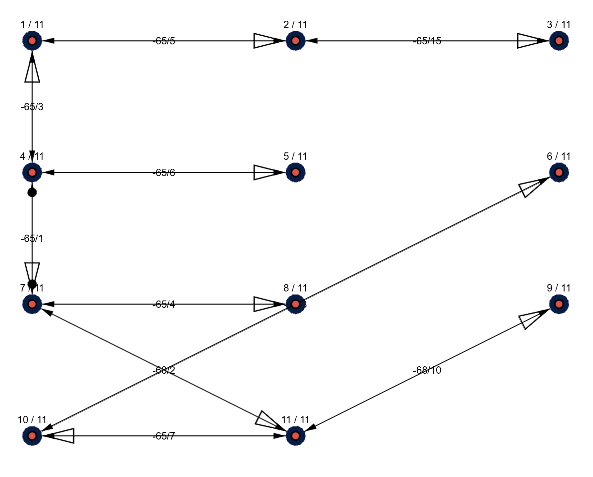
\includegraphics[width = 0.6\textwidth]{image/模擬實驗11點seed=1.png}
    \caption{模擬節點數量=11點,Seed=1}
    \label{fig: 模擬實驗11點seed=1}
\end{figure}

\begin{figure}[H]
    \centering
    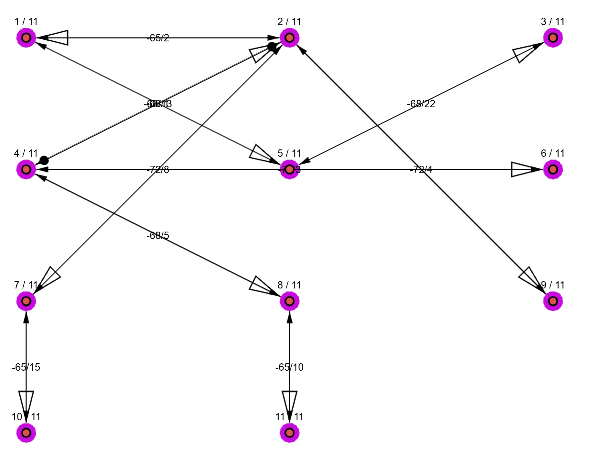
\includegraphics[width = 0.6\textwidth]{image/模擬實驗11點seed=10.png}
    \caption{模擬節點數量=11點,Seed=10}
    \label{fig: 模擬實驗11點seed=10}
\end{figure}

\begin{figure}[H]
    \centering
    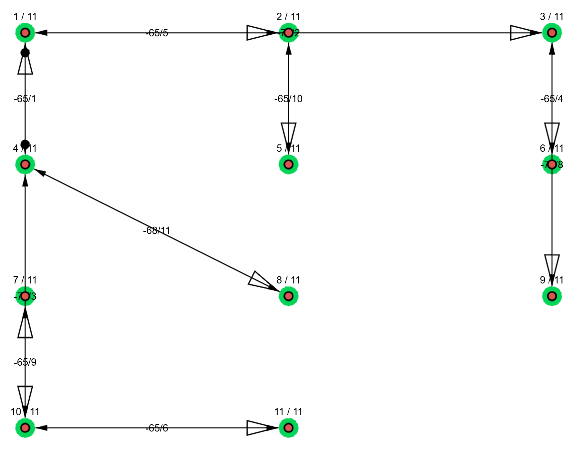
\includegraphics[width = 0.6\textwidth]{image/模擬實驗11點seed=100.png}
    \caption{模擬節點數量=11點,Seed=100}
    \label{fig: 模擬實驗11點seed=100}
\end{figure}

\begin{figure}[H]
    \centering
    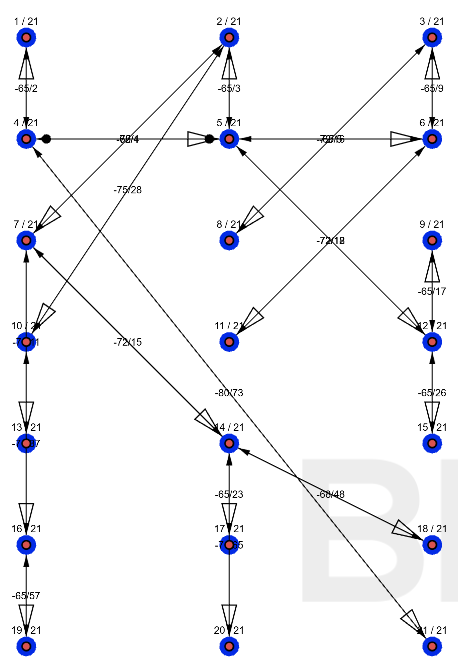
\includegraphics[width = 0.6\textwidth]{image/模擬實驗21點seed=1.png}
    \caption{模擬節點數量=21點,Seed=1}
    \label{fig: 模擬實驗21點seed=1}
\end{figure}

\begin{figure}[H]
    \centering
    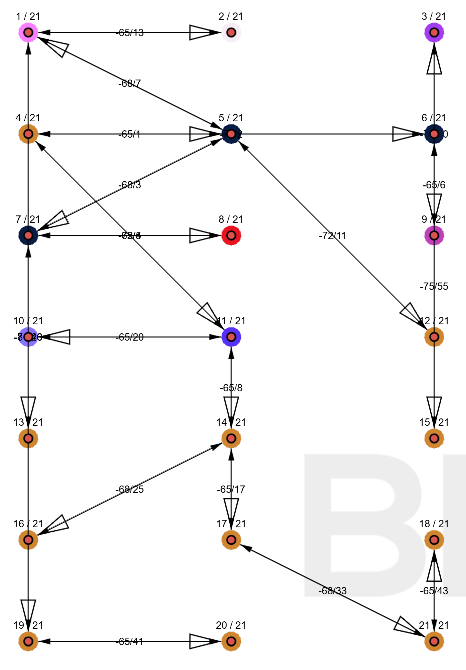
\includegraphics[width = 0.6\textwidth]{image/模擬實驗21點seed=10.png}
    \caption{模擬節點數量=21點,Seed=10}
    \label{fig: 模擬實驗21點seed=10}
\end{figure}

\begin{figure}[H]
    \centering
    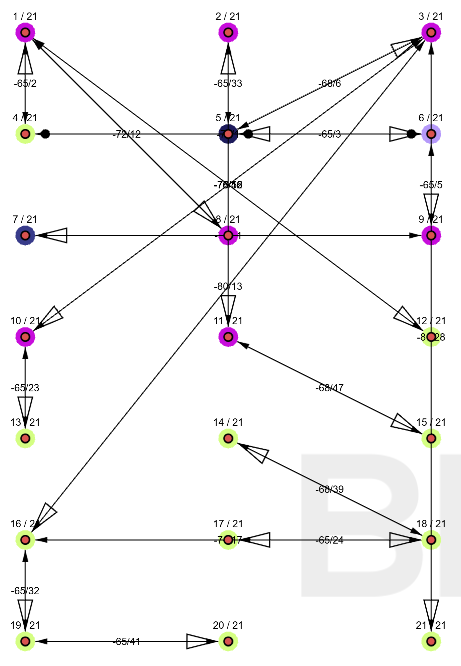
\includegraphics[width = 0.6\textwidth]{image/模擬實驗21點seed=100.png}
    \caption{模擬節點數量=21點,Seed=100}
    \label{fig: 模擬實驗21點seed=100}
\end{figure}

\begin{figure}[H]
    \centering
    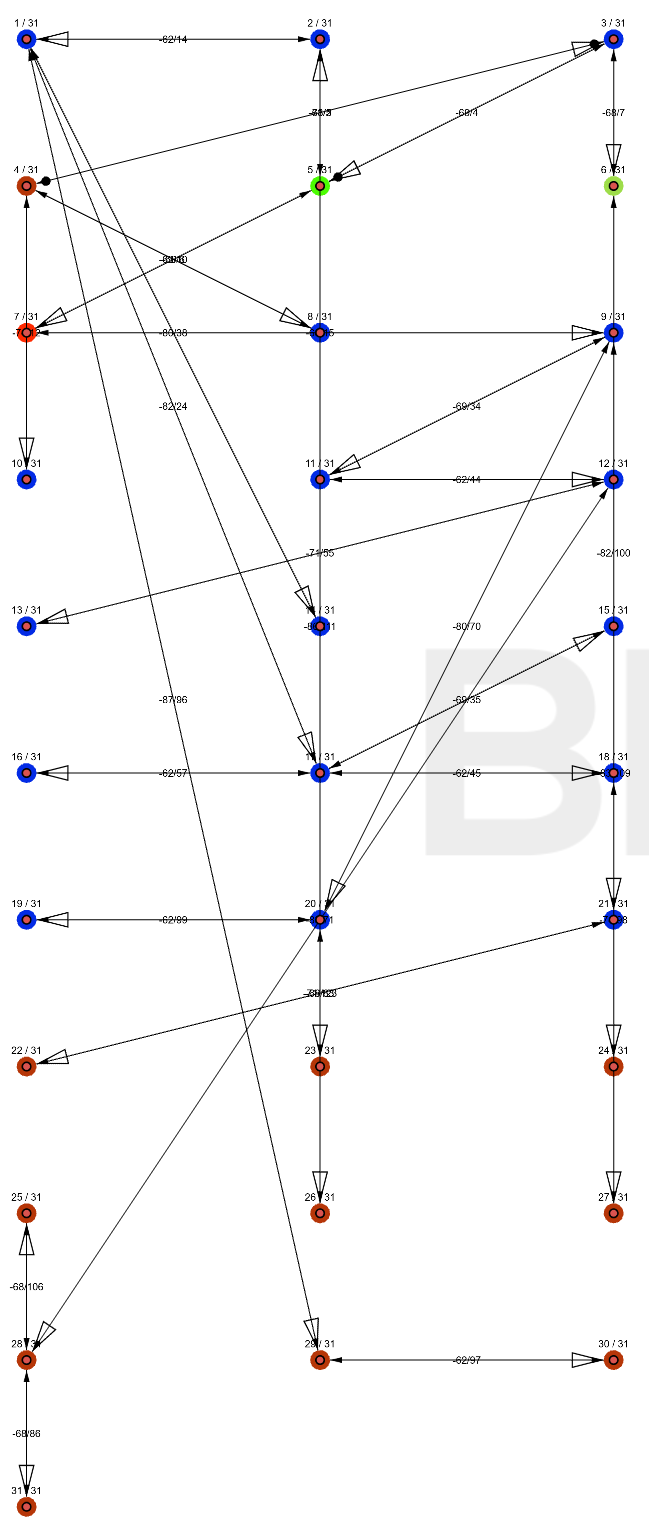
\includegraphics[width = 0.6\textwidth]{image/模擬實驗31點seed=1.png}
    \caption{模擬節點數量=31點,Seed=1}
    \label{fig: 模擬實驗31點seed=1}
\end{figure}

\begin{figure}[H]
    \centering
    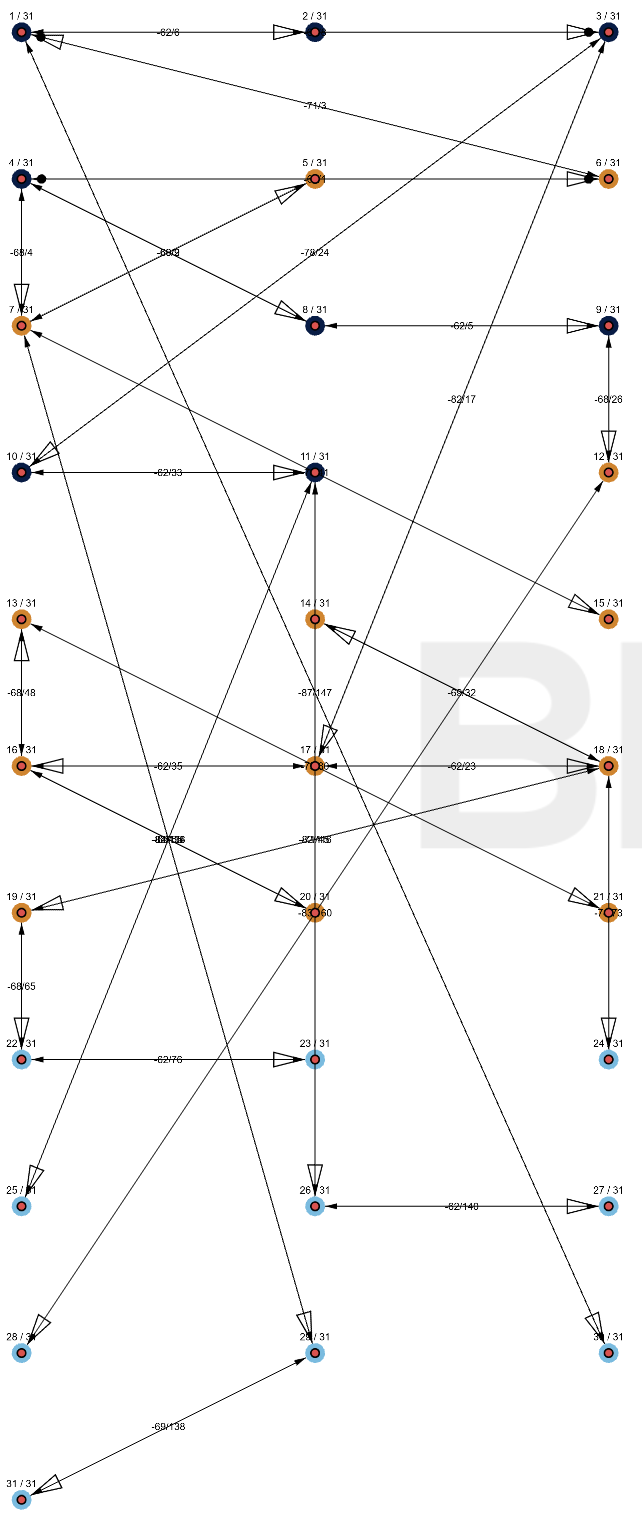
\includegraphics[width = 0.6\textwidth]{image/模擬實驗31點seed=10.png}
    \caption{模擬節點數量=31點,Seed=10}
    \label{fig: 模擬實驗31點seed=10}
\end{figure}

\begin{figure}[H]
    \centering
    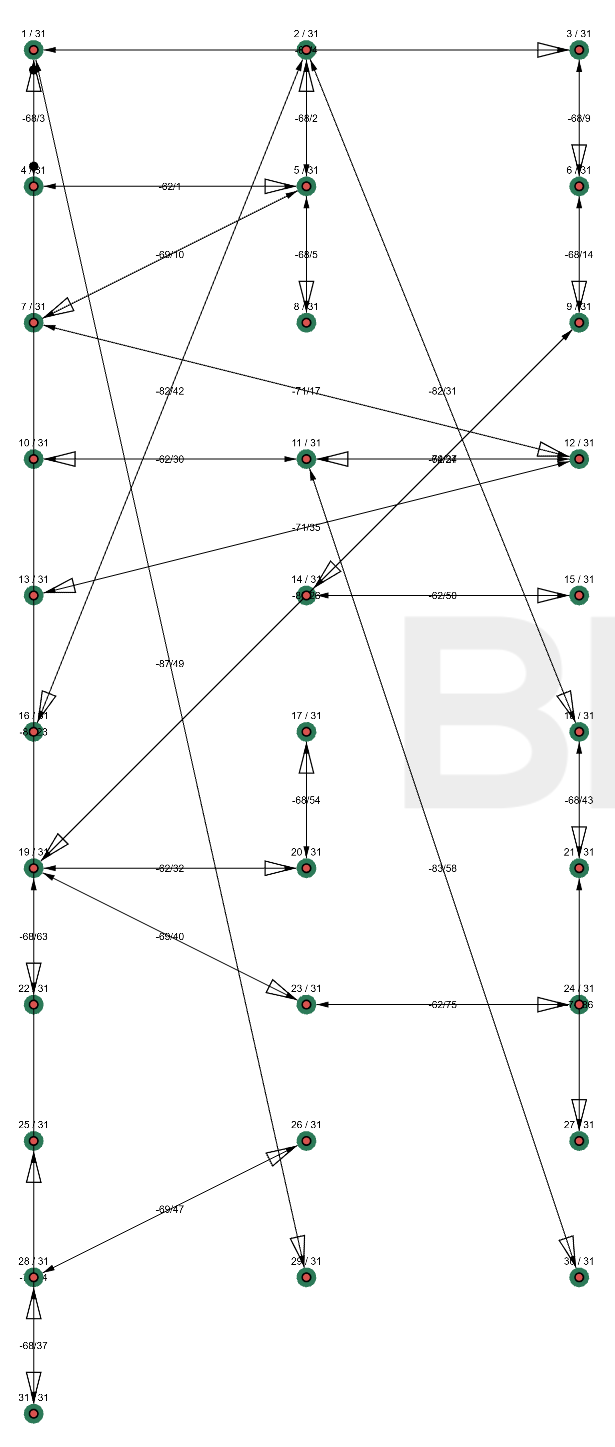
\includegraphics[width = 0.6\textwidth]{image/模擬實驗31點seed=100.png}
    \caption{節點數量=31點,Seed=100}
    \label{fig: 模擬實驗31點seed=100}
\end{figure}

\subsection{模擬提出之網路拓樸Sink 節點斷線後拓樸重建機制}
模擬實驗中,會將 Sink 節點斷線後,Mesh系統能夠自動重新建立拓樸並確保 Sink 節點仍然是根節點。分別以節點數量11、21及31實驗10次,圖\ref{fig: 模擬實驗11點sink斷線後連回}、\ref{fig: 模擬實驗21點sink斷線後連回}及\ref{fig: 模擬實驗31點sink斷線後連回}分別顯示了節點數量為11、21及31時,Sink節點(節點位置4)斷線後重新連線後的結果。可以觀察到,即使在 Sink 節點斷線後,Mesh系統仍能恢復並保持Sink節點(節點位置4)在拓樸的根節點。

\begin{figure}[H]
    \centering
    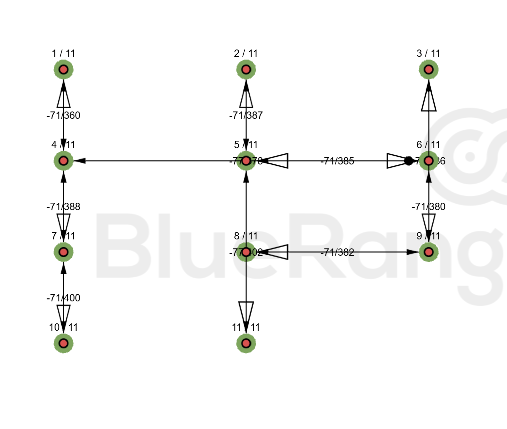
\includegraphics[width = 0.8\textwidth]{image/模擬實驗11點sink斷線後連回.png}
    \caption{模擬實驗11點sink斷線後連回結果}
    \label{fig: 模擬實驗11點sink斷線後連回}
\end{figure}

\begin{figure}[H]
    \centering
    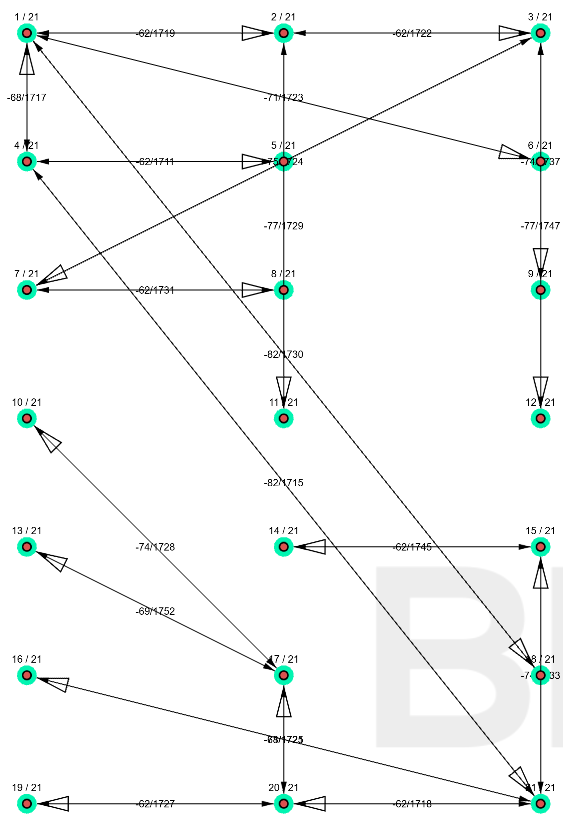
\includegraphics[width = 0.8\textwidth]{image/模擬實驗21點sink斷線後連回.png}
    \caption{模擬實驗21點sink斷線後連回結果}
    \label{fig: 模擬實驗21點sink斷線後連回}
\end{figure}

\begin{figure}[H]
    \centering
    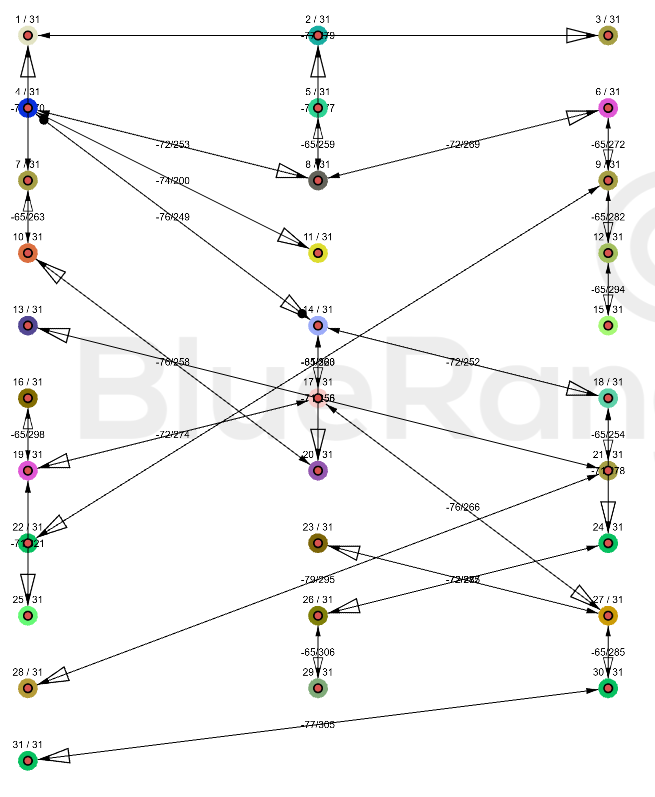
\includegraphics[width = 0.6\textwidth]{image/模擬實驗31點sink斷線後連回.png}
    \caption{模擬實驗31點sink斷線後連回結果}
    \label{fig: 模擬實驗31點sink斷線後連回}
\end{figure}


\subsection{模擬節點重啟後之拓樸重建時間分析}
在本研究中,為驗證所提出機制於節點重啟(reset)後的拓樸重建效率,設計了不同網路規模下的模擬實驗。實驗分別針對節點總數為 11、21 及 31 的網路拓樸進行,並比較兩種節點類型的重啟情境,分別為 Sink 節點(根節點)與非 Sink 節點(一般中繼節點或邊緣節點)。

每一種網路規模與節點類型情境下,皆進行 100 次重啟測試,記錄節點自啟動至成功連入 Mesh 網路所需之時間,並據此計算其平均連線時間與標準差。其中,針對非 Sink 節點的測試情境,於每次重啟實驗中均隨機選擇一個非 Sink 節點進行重啟,以更真實模擬實際網路環境中任意節點故障後的恢復行為。

透過大量重複實驗,能更準確評估系統在拓樸變動下的穩定性與恢復能力,並觀察不同節點角色對 Mesh 重建效率的影響。本實驗分別於 11 點、21 點與 31 點之網路拓樸規模下,針對 Sink 節點與非 Sink 節點進行模擬測試。每組情境皆重複執行 100 次實驗,統計其 Mesh 成功建立所需的平均時間與標準差,結果如圖 \ref{fig: 節點重啟後之拓樸重建時間分析} 所示。

\begin{figure}[H]
    \centering
    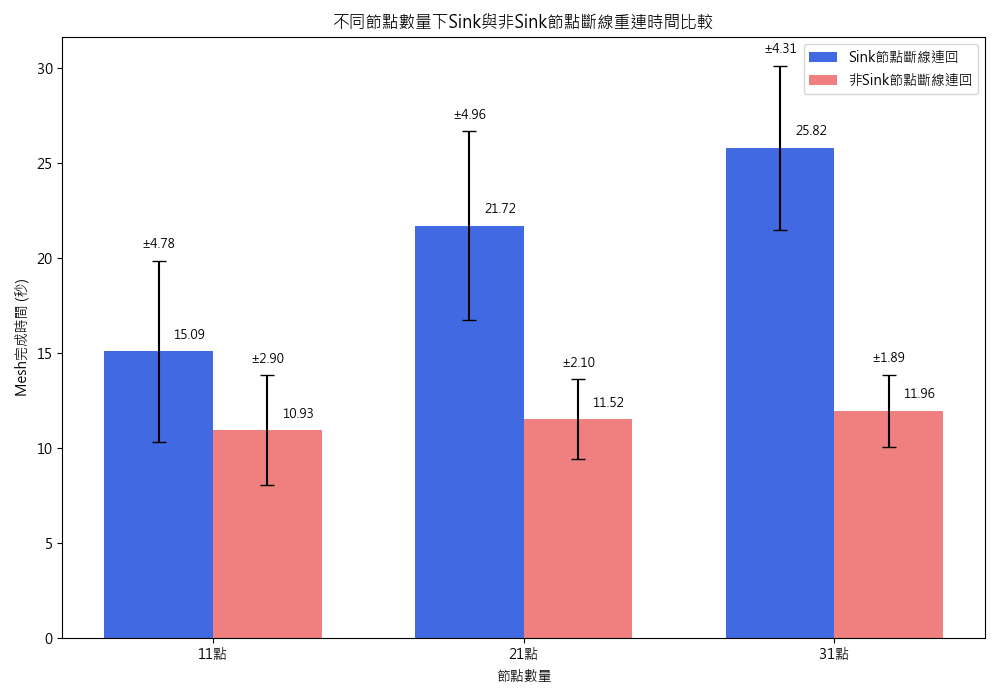
\includegraphics[width = 1\textwidth]{image/補實驗節點重啟後之拓樸重建時間分析.png}
    \caption{模擬節點重啟後之拓樸重建時間分析}
    \label{fig: 節點重啟後之拓樸重建時間分析}
\end{figure}

從實驗結果可觀察到,在三種網路規模下,非 Sink 節點的重啟連線平均時間皆維持在約 10.93~11.96 秒之間,且標準差相對較小,大約 1.89~2.9,顯示其連線行為穩定且具一致性。而相較之下,Sink 節點的重啟平均時間顯著較高,分別為 15.09 秒(11 點)、21.72 秒(21 點)與 25.82 秒(31 點),且標準差相對比較大(約 4.31~4.96),顯示在重建根節點角色與拓樸過程中,其恢復行為具有較高的變異性與延遲風險。

此現象可歸因於 Sink 節點在拓樸中需重新扮演根節點角色,並建立樹狀結構的主幹連線路徑,因此重啟後需耗費較多時間進行握手、選擇路徑與節點重連。此外,實驗亦證實所提出之拓樸修復機制能在重啟後正確辨識 Sink 節點並讓其重新成為 Mesh 拓樸的根節點,保持網路層級的一致性與穩定性。

\subsection{模擬不同節點數與隨機環境下拓樸平衡性分析}
本節實驗針對原生 FruityMesh 與本研究所提出之修改後演算法在所建立的網路拓樸平衡性上的表現進行比較。拓樸平衡性的衡量方式以節點連向 Sink 節點所需跳數(HopsToSink)作為評估依據,平均值與最大值越低表示拓樸越平衡、傳輸路徑越有效率。

模擬實驗中,模擬建立的網路拓樸皆以 節點位置4 作為 Sink 節點 ,分別使用 11、21 及 31 節點進行測試,並針對每種節點數量採用 10 次隨機 Seed ,來模擬不同的網路拓樸建立情形。每次模擬均記錄節點到 Sink 節點的平均 HopsToSink 與最大 HopsToSink 值,並計算11、21 及 31 節點平均結果,以評估拓樸平衡性。
實驗結果如圖 \ref{fig: Avg_hops_comparison} 及 \ref{fig: Max_hops_comparison} 所示,分別列出原生 FruityMesh 與本研究所提出之演算法在不同節點數量下所建立網路拓樸的平均與最大 HopsToSink 值。
從平均結果可見,修改版本在各節點數情境中皆展現出更佳的拓樸平衡性。在節點數為 11 的情況下,平均HopsToSink由原生版本的 2.699 降至修改版本的 2.009,最大HopsToSink亦由 4.8 降至 3.8,顯示節點能以更短的路徑連接至 Sink 節點。當節點數增加至 21 時,修改版本同樣表現穩定,平均HopsToSink由 3.524 降至 2.923,最大HopsToSink由 6.5 降為 5.7。即使在節點數量較高的 31 點情境中,修改版本亦可將平均HopsToSink由 4.673 有效降低至 3.561,最大HopsToSink亦由 8.2 降至 6.7。

\begin{figure}[H]
    \centering
    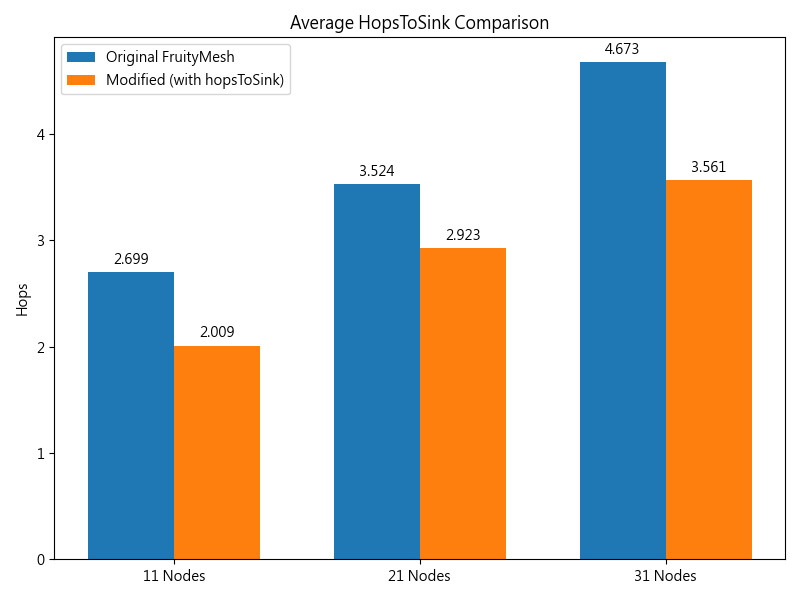
\includegraphics[width = 0.8\textwidth]{image/Avg_hops_comparison.png}
    \caption{平均HopsToSink比較}
    \label{fig: Avg_hops_comparison}
\end{figure}

\begin{figure}[H]
    \centering
    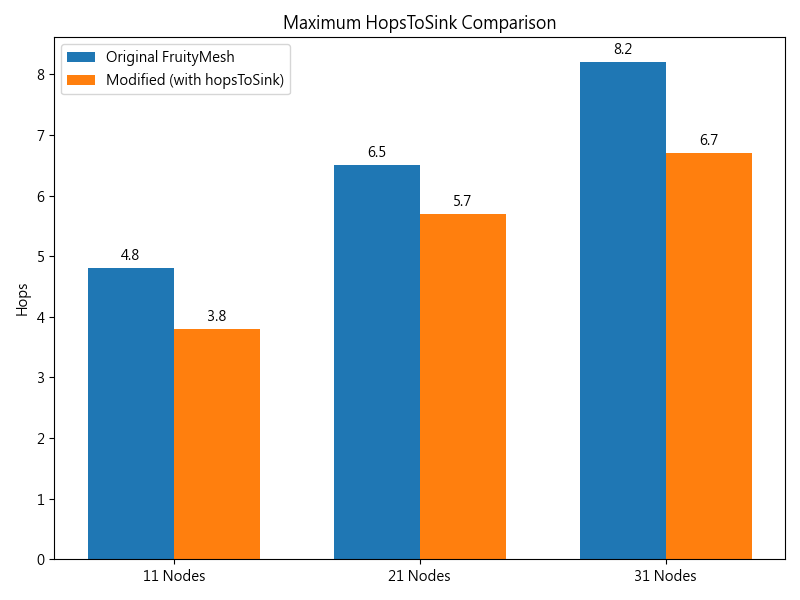
\includegraphics[width = 0.8\textwidth]{image/Max_hops_comparison.png}
    \caption{最大HopsToSink比較}
    \label{fig: Max_hops_comparison}
\end{figure}

\subsection{實作提出之網路拓樸建立}
實體實驗中,使用 6塊 Nordic nRF52840-DK 開發板進行小規模拓樸建立測試,表\ref{tab: 實作提出之網路拓樸建立參數設定}為相關參數設定。每個節點均配置為 FruityMesh 協定堆疊,並透過 UART 進行日誌紀錄。

\begin{table}[H]
    \centering
    \caption{實作提出之網路拓樸建立參數設定}
    \label{tab: 實作提出之網路拓樸建立參數設定}
    \begin{tabular}{|c|c|}
        \hline
        參數名稱 & 設定值 \\
        \hline
        節點數量 & 6(包含1個Sink節點) \\
        \hline
        Sink 節點編號 & 1 / 5 \\
        \hline
        Connection Interval & 100 ms \\
        \hline
        Connection Event & 10 ms \\
        \hline
    \end{tabular}
\end{table}

\subsubsection{實作初始化拓樸中Sink點之Root角色實驗}
為驗證本研究所提出的拓樸建立機制是否能正確地將指定之 Sink 節點設定為整個 BLE Mesh 網路的 Root(根節點),本實驗設計兩組不同的節點配置情境進行觀察。每組實驗均包含 6 個 nRF52840 節點,其中僅指定其中一節點為 Sink,其餘皆設定為 Static 類型,並透過 UART 回傳每個節點之拓樸連線資訊,以視覺化方式呈現網路結構。

在第一組實驗中,節點編號為 1(nodeId = 1)者被指定為 Sink 節點,初始化完成後之網路拓樸如圖 \ref{fig: 實作sink=1初始化拓樸圖} 所示。從拓樸圖可觀察到,所有節點皆透過多層結構連接至節點 1,且未出現多個中心節點或分離子網情形,顯示該節點成功成為整體 Mesh 的根節點。

\begin{figure}[H]
    \centering
    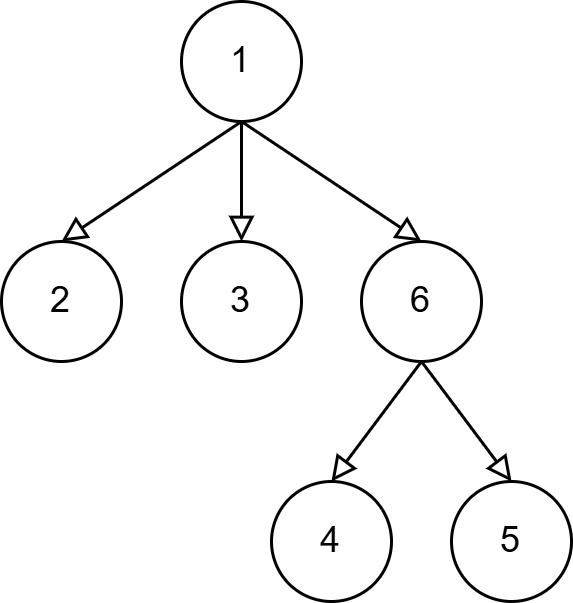
\includegraphics[width = 0.3\textwidth]{image/實作sink=1初始化拓樸圖.jpg}
    \caption{實作sink=1初始化拓樸圖}
    \label{fig: 實作sink=1初始化拓樸圖}
\end{figure}

於第二組實驗中,改由節點 5(nodeId = 5)作為 Sink,其他節點仍為 Static。初始化後之連線關係如圖 \ref{fig: 實作sink=5初始化拓樸圖} 所示,同樣可觀察到所有節點皆以節點 5 為樞紐,逐層建立向外擴展之拓樸,符合樹狀結構設計原則,Sink 成功成為網路中心。

\begin{figure}[H]
    \centering
    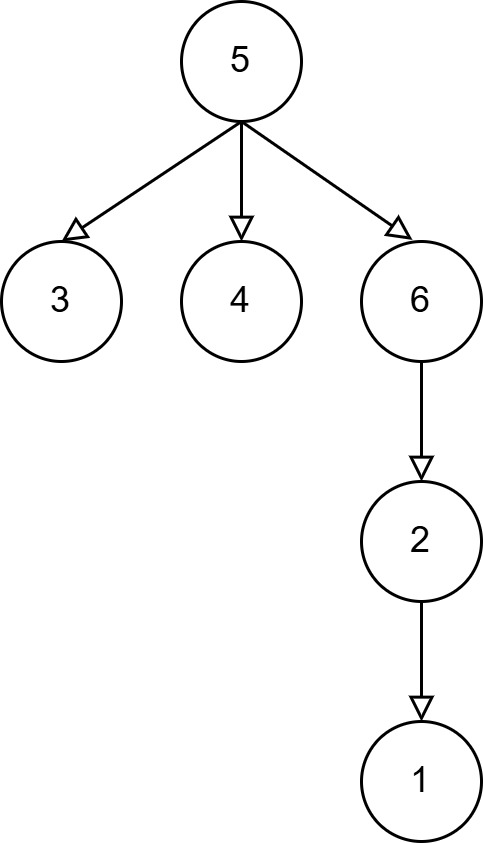
\includegraphics[width = 0.3\textwidth]{image/實作sink=5初始化拓樸圖.jpg}
    \caption{實作sink=5初始化拓樸圖}
    \label{fig: 實作sink=5初始化拓樸圖}
\end{figure}

此兩組實驗皆證實,本研究所實作之拓樸建立演算法在初始化階段能正確識別 Sink 節點,並將其設為網路的 Root。即使在不同位置指定 Sink 節點(如節點 1 或 5),皆可以達到以 Sink 為Root之拓樸結構。

\subsubsection{實作重啟拓樸中Sink點之Root角色實驗}
在本實驗中,針對已建立之 BLE Mesh 拓樸進行節點重啟測試,以驗證系統在節點重啟後能否正確恢復拓樸結構並保持 Sink 節點的 Root 角色。實驗中,分別將節點 1 及 節點 5 設定為 Sink 節點,並透過 USB 日誌紀錄方式觀察其連線狀態。

在節點 1 為 Sink 節點的情境中,當其重新啟動Sink節點後,BLE Mesh 系統能夠自動重新建立拓樸結構,並正確地維持節點 1 為整體網路的根節點。圖 \ref{fig: 實作sink=1初始化拓樸圖} 與圖 \ref{fig: 實作sink=1重啟拓樸圖} 分別顯示拓樸初始化與節點 1 重啟後的拓樸變化情形。

從圖中可觀察到,初始化時節點 2、3、6 為節點 1的子節點,節點 4、5 為節點 6 的子節點;而在重啟後,節點 2、4、6 為節點 1 的直接子節點,節點 3、5 成為節點 6 的子節點,其中節點 3 則改為節點 6 的子節點,且節點 4 作為節點 1 的子節點。



%在節點 1 重啟後,系統能夠自動重新建立拓樸,並確保節點 1 仍然是整個 Mesh 網路的根節點。圖 \ref{fig: 實作sink=1重啟拓樸圖} 顯示了重啟後的拓樸結構,從中可見所有節點仍然以節點 1 為根節點,完成拓樸建立。

\begin{figure}[H]
    \centering
    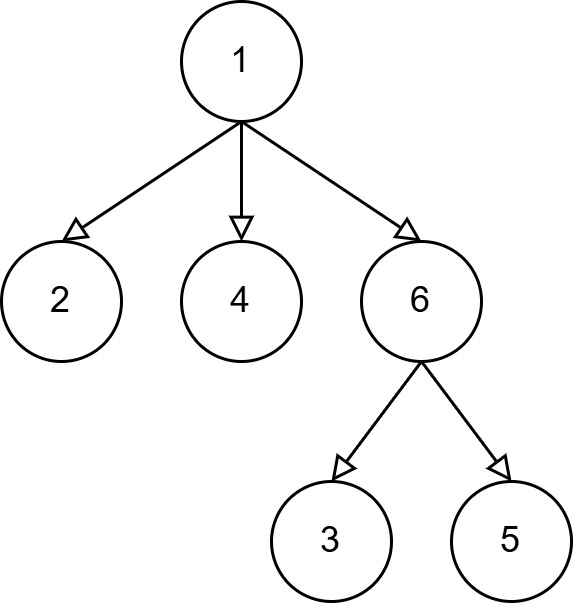
\includegraphics[width = 0.3\textwidth]{image/實作sink=1重啟拓樸圖.jpg}
    \caption{實作sink=1重啟拓樸圖}
    \label{fig: 實作sink=1重啟拓樸圖}
\end{figure}

在節點 5 為 Sink 節點的情境中,當其重新啟動Sink節點後,BLE Mesh 系統能夠自動重新建立拓樸結構,並正確地維持節點 5 為整體網路的根節點。圖 \ref{fig: 實作sink=5初始化拓樸圖} 與圖 \ref{fig: 實作sink=5重啟拓樸圖} 分別顯示拓樸初始化與節點 5 重啟後的拓樸變化情形。

從圖中可觀察到,初始化時節點 2、3、6 直接連接至節點 5,節點 1 為節點 3 的子節點,節點 4 則為節點 6 的子節點;而在重啟後,節點 4、6 為節點 5 的直接子節點,節點 3 成為節點 4 的子節點,節點 1 則改為節點 6 的子節點,並新增節點 2 作為節點 1 的子節點。

儘管連線路徑出現變動,整體 Mesh 拓樸仍以 Sink 節點為網路的根節點,驗證了本研究提出之拓樸穩定性與 Sink 節點斷線重連機制的有效性。

%在節點 5 為Sink節點重啟,BLE Mesh重新建立拓樸結構後,節點 5 依然為整個BLE Mesh的根節點。從圖 \ref{fig: 實作sink=5初始化拓樸圖} 與圖 \ref{fig: 實作sink=5重啟拓樸圖} 可見,重啟前後的網路拓樸結構一致,各節點的連線關係保持穩定,節點 3、4、6 皆直接連接至節點 5,節點 2 及節點 1 亦維持在原有層級位置。

\begin{figure}[H]
    \centering
    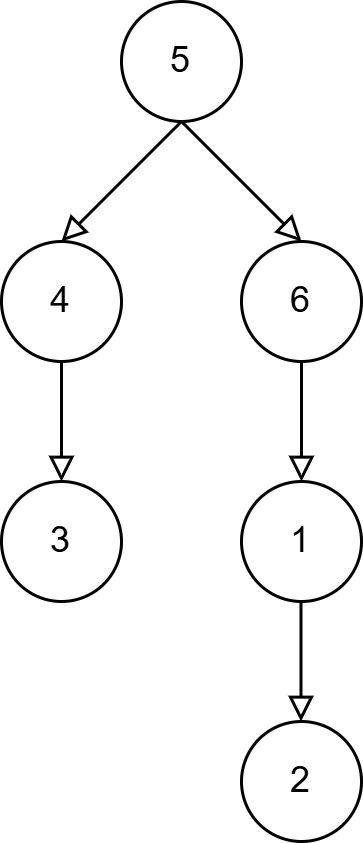
\includegraphics[width = 0.2\textwidth]{image/實作sink=5重啟拓樸圖.jpg}
    \caption{實作sink=5重啟拓樸圖}
    \label{fig: 實作sink=5重啟拓樸圖}
\end{figure}

這些變化反映出在 BLE Mesh 網路中,拓樸會根據各節點連線狀態與可用性進行自我調整,以建立最合適的路徑結構。儘管節點間的連線順序與位置改變,Mesh 系統仍能確保 Sink 節點保持 Root 身份,且整體網路架構維持完整,展現出所提機制在拓樸重建過程中的穩定性與靈活性。

\section{層級式 Connection Interval 機制之效能比較分析}
實驗採用與文獻 \cite{112TIT00392032} 相同之實體拓樸架構,如圖 \ref{fig: 實體拓樸架構} 所示。然而,相較於文獻 \cite{112TIT00392032} 於所有節點均採用固定 Connection Interval(CI)設定之方式,本研究進一步提出「分層調整 CI」之機制,依節點於拓樸中所處層級設定不同的連線間隔時間,讓越接近Sink點的節點,因為負載量提高,藉由縮短Connection Interval(CI),提高所配置的頻寬,同時就可以有更多向Sink節點傳輸的時間,以提升整體網路穩定性。
整體網路包含六個節點,並採用樹狀拓樸設計,各節點之 Connection Interval(CI)依其所處層級進行遞增設置,從 Sink 節點 至 末端節點,分別依序設置 CI = 25 ms、CI = 50 ms 及 CI = 100 ms。

\begin{figure}[H]
    \centering
    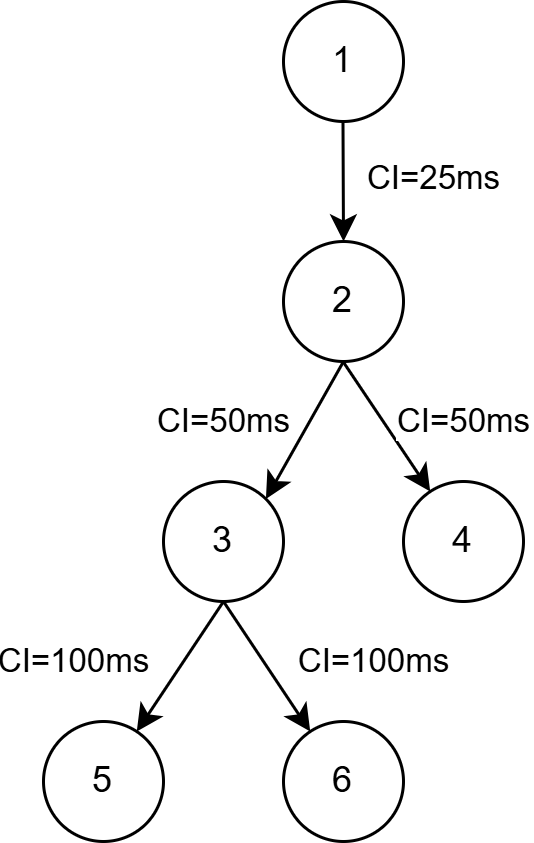
\includegraphics[width = 0.3\textwidth]{image/BLE Mesh封包傳輸機制設計節點架構圖.png}
    \caption{實體拓樸架構}
    \label{fig: 實體拓樸架構}
\end{figure}

本實驗採用六個節點所構成之靜態樹狀拓樸架構,並以 Nordic nRF52840-DK 開發板進行節點間實際通訊連線。節點間距小於 1 公尺,所有節點均透過 UART 介面回傳即時封包傳輸紀錄與通訊延遲,以便後續進行統計分析。相關實驗參數設定詳如表 \ref{tab: 實體拓樸架構實驗參數設定} 所示。

\begin{table}[H]
    \centering
    \caption{實體拓樸架構實驗參數設定}
    \label{tab: 實體拓樸架構實驗參數設定}
    \begin{tabular}{|c|c|}
        \hline
        參數名稱 & 設定值 \\
        \hline
        Number of nodes & 6(including 1 Sink) \\
        \hline
        Sink NodeId & 1 \\
        \hline
        Distance between nodes & < 1m \\
        \hline
        Connection Interval & 25 ms(Sink), 50 ms(1st hop), 100 ms(2nd hop) \\
        \hline
        Scan Interval & 25 ms(Sink), 50 ms(1st hop), 100 ms(2nd hop)\\
        \hline
        Connection Event & 10 ms \\
        \hline
        Packet Amount & 25, 50, 75, 100 packet/ node \\
        \hline
        Packet Rate & 1 packet / 100ms \\
        \hline
        Payload Size & 30 bytes \\
        \hline
    \end{tabular}
\end{table}

在連線設定方面,Sink 節點(節點 1)配置最短之 Connection Interval 為 25 ms,而其他節點則依其拓樸中所處層級遞增調整,第一層(1-hop)為 50 ms,第二層(2-hop)為 100 ms,且Scan Interval(SI)時間皆與CI設定值相同。此分層設定的目的在於分散不同節點的通訊時間,可以讓越接近Sink點的節點有夠多傳輸的時間,進而提升封包傳輸的穩定性與效率。

在資料傳輸設定部分,各節點分別傳送 25、50、75 及 100 筆封包,模擬不同傳輸封包總量下的傳輸表現。每筆封包大小為 30 bytes,封包發送頻率固定為每 100 ms 傳送一筆。為使實驗結果具一致性,所有節點會同步開始傳送資料至 Sink 節點,並於每次連線事件間隔(Connection Event)設為 10 ms 的條件下完成通訊流程。

透過上述實體參數設定,得以在受控環境下有效觀察分層 Connection Interval 對藍牙 Mesh 網路中封包延遲、重傳率及傳輸成功率等指標之實際影響,並進一步與固定 Connection Interval 設定之傳統方法進行比較分析,以驗證本研究機制之優勢與實用性。

\subsection{平均封包延遲比較}
圖 \ref{fig: avg_delay} 為不同封包發送數量下,各機制所產生之平均封包延遲時間結果。由圖可觀察到,FruityMesh 原生機制在負載增加時延遲呈現明顯上升趨勢,從 966.07 ms 增加至 1734.08 ms;DOST 機制雖略有改善,但延遲仍達 978.05 ms。而本研究所提出之層級式 CI 調整機制,在四種傳輸量條件下皆能穩定維持低延遲表現,延遲平均均維持約為 175 ms 左右,顯示該機制可有效降低傳輸碰撞與佇列等待時間,提升即時性表現,並維持系統的穩定。

\begin{figure}[H]
    \centering
    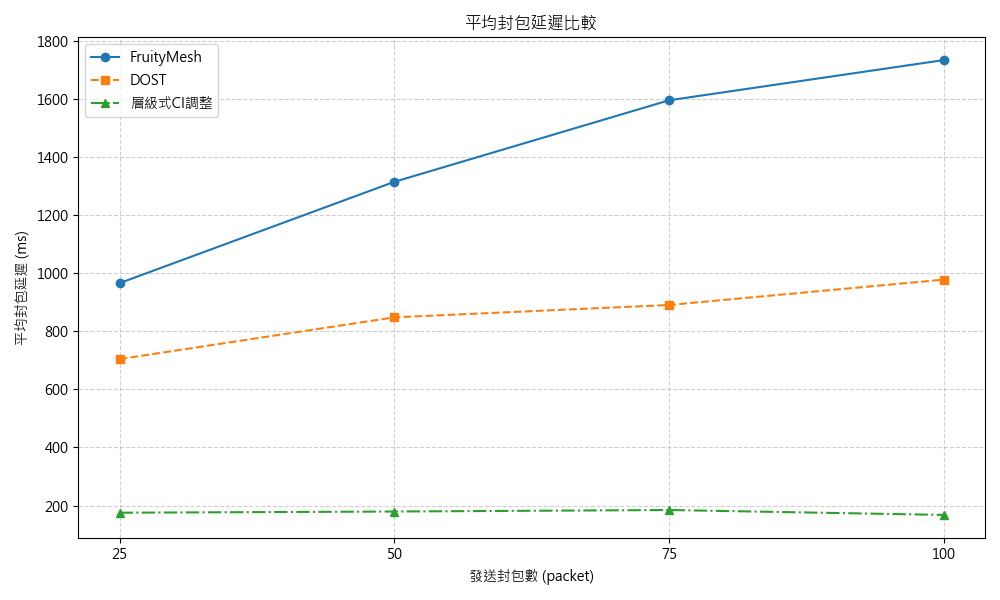
\includegraphics[width = 0.8\textwidth]{image/Avg_Packet_Delay_Comparison.png}
    \caption{平均封包延遲比較}
    \label{fig: avg_delay}
\end{figure}

\subsection{平均封包重傳率比較}
圖 \ref{fig: avg_retrans} 顯示不同機制在各封包數下之平均重傳率變化。原生 FruityMesh 在高傳輸量情境下重傳率明顯偏高,甚至超過 100\%,表示多數封包需多次嘗試方能成功送達,造成網路擁塞與效能下降,系統趨向不穩定。DOST 機制的重傳率維持在 14\% 至 19\% 之間,雖低於 FruityMesh,仍顯示網路存在傳輸瓶頸。而本研究所提方法在所有負載下之重傳率皆低於 1.3\%,其中最低僅 0.07\%,顯示其具備優異的穩定性與傳輸效率。

\begin{figure}[H]
    \centering
    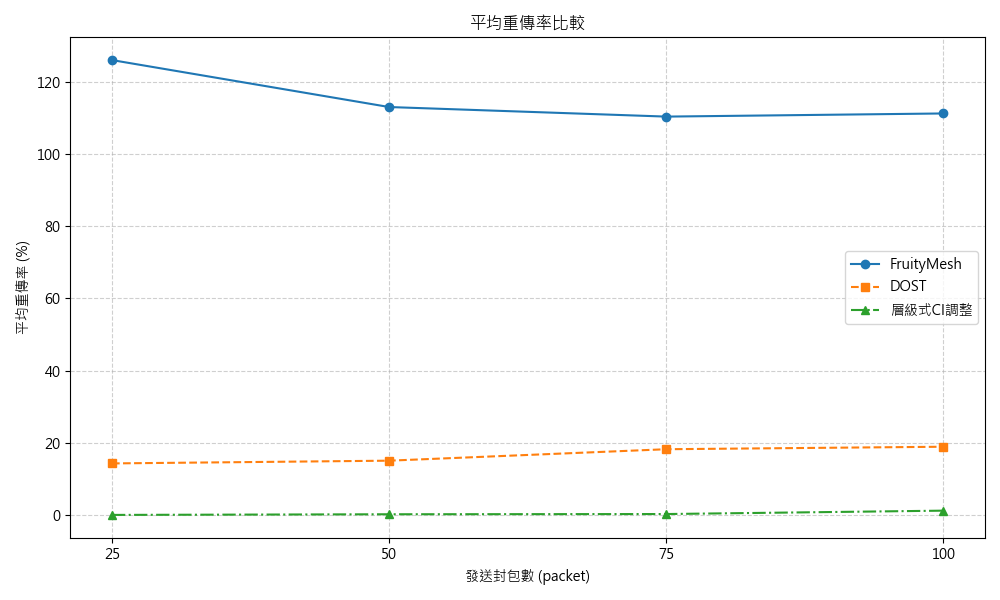
\includegraphics[width = 0.8\textwidth]{image/Avg_Retransmission_Rate_Comparison.png}
    \caption{平均封包重傳率比較}
    \label{fig: avg_retrans}
\end{figure}

\subsection{平均封包傳輸成功率比較}
圖 \ref{fig: pdr} 比較三種機制在不同封包數量下的封包傳輸成功率表現。FruityMesh 的 PDR 隨封包數增加明顯下降,從 99\% 降至 73.08\%,呈現明顯的退化及不穩定趨勢。DOST 機制與本研究提出之層級式 CI 調整機制則在各情境下皆維持 100\% 的封包傳輸成功率,顯示後兩者在處理高負載傳輸時能有效避免封包遺失,維持高度的通訊可靠性。

\begin{figure}[H]
    \centering
    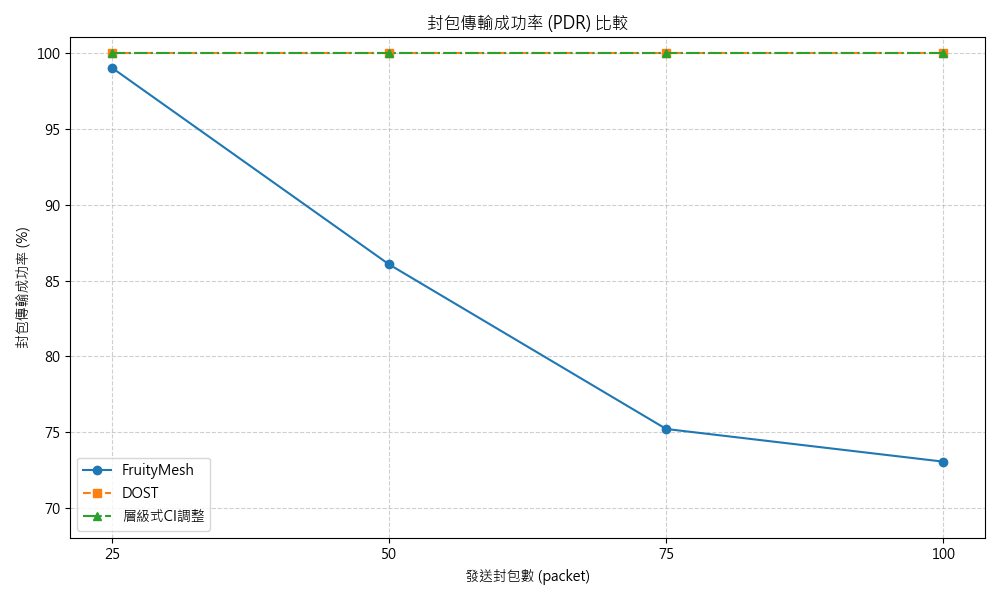
\includegraphics[width = 0.8\textwidth]{image/PDR_Comparison.png}
    \caption{平均封包傳輸成功率比較}
    \label{fig: pdr}
\end{figure}

\end{ZhChapter}